
% Copyright 2004 by Till Tantau <tantau@users.sourceforge.net>.
%
% In principle, this file can be redistributed and/or modified under
% the terms of the GNU Public License, version 2.
%
% However, this file is supposed to be a template to be modified
% for your own needs. For this reason, if you use this file as a
% template and not specifically distribute it as part of a another
% package/program, I grant the extra permission to freely copy and
% modify this file as you see fit and even to delete this copyright
% notice. 

\documentclass{beamer}

\usetheme{Madrid}
\usepackage[lithuanian]{babel}
\usepackage[utf8x]{inputenc}
\def\LTfontencoding{L7x}
\usepackage{times}
\usepackage[T1]{fontenc}
\usepackage{color}
\usepackage{verbatim}
\usepackage{graphicx}
\usepackage{fancyvrb}
\usepackage{bm}
\usepackage{amsfonts}
\usepackage{hyperref}
\usepackage{caption}
\usepackage{subfig}
\usepackage{comment}
\usepackage{minted}
\usepackage{hyperref}
\usepackage{animate}
\usepackage{tikz}

\title{Technologijos, kurias galima panaudoti mokyme. 1 dalis}
\author{Simonas Mamaitis}
\institute[VU]
{VU\\
}
\date{2019 Birželis}



% Let's get started
\begin{document}

\begin{frame}
  \titlepage
\end{frame}

\begin{frame}
Šioje dalyje bus pademonstruojamos technologijos, kurias galima panaudoti aiškinant matematinę medžiagą:
\begin{itemize}
\item Vizualizacijos, prieinamos kuriant .pdf failus per Latex skriptą
\end{itemize}
\end{frame}

\begin{frame}[fragile]{Sprendimų vaizdavimas su .pdf failais}
1. Uždavinių sprendimų automatizavimas su Python
\begin{itemize}
\item Tikslas: palengvinti kelią mokantis matematines procedūras.
\item Uždavinys būna žinomas. Pvz. išspręsti lygčių sistemą Gauso metodu.
\item Į aplinką įvedami pradiniai duomenys.
\item Programa sugeneruoja sprendimą .tex formatu
\item Sprendimą vėliau rankiniu būdu arba automatiškai galima versti į .pdf failą.
\end{itemize}
\end{frame}

\begin{frame}[fragile]{Automatizavimo pavyzdys}
 Lygčių sistemos sprendimas Gauso metodu.
$\left\{\begin{array}{lr}
1a + 1b + 2c + 1d &=7\\
3a + 4b + 8c + 5d &=29\\
1a + 3b + 7c + 8d &=30\\
2a + 2b + 5c + 6d &=23\\
\end{array}\right.$
\end{frame}

\begin{frame}[fragile]{Automatizavimo pavyzdys}
\noindent$\left(\begin{array}{rrrr|r}
\bm{1} & \bm{1} & \bm{2} & \bm{1} & \bm{7}\\
\textcolor{blue}{3} & 4 & 8 & 5 & 29\\
\textcolor{blue}{1} & 3 & 7 & 8 & 30\\
\textcolor{blue}{2} & 2 & 5 & 6 & 23\\
\end{array}\right)
\setlength{\unitlength}{1pt}
\begin{picture} (95, 0)
\put(0.0, 21.0){\vector(0, -1){12}}
\put(3.0, 15.0){\tiny{$\times\left(-3\right)$}}
\put(35.0, 21.0){\vector(0, -1){24}}
\put(38.0, 15.0){\tiny{$\times\left(-1\right)$}}
\put(70.0, 21.0){\vector(0, -1){36}}
\put(73.0, 15.0){\tiny{$\times\left(-2\right)$}}
\end{picture}=$
\end{frame}

\begin{frame}[fragile]{Automatizavimo pavyzdys}
\noindent$\left(\begin{array}{rrrr|r}
1 & 1 & 2 & 1 & 7\\
\bm{0} & \bm{1} & \bm{2} & \bm{2} & \bm{8}\\
0 & \textcolor{blue}{2} & 5 & 7 & 23\\
0 & \textcolor{blue}{0} & 1 & 4 & 9\\
\end{array}\right)
\setlength{\unitlength}{1pt}
\begin{picture} (95, 0)
\put(0.0, 9.0){\vector(0, -1){12}}
\put(3.0, 3.0){\tiny{$\times\left(-2\right)$}}
\put(35.0, 9.0){\vector(0, -1){24}}
\put(38.0, 3.0){\tiny{$\times\left(0\right)$}}
\end{picture}=$
\end{frame}

\begin{frame}[fragile]{Automatizavimo pavyzdys}
\noindent$\left(\begin{array}{rrrr|r}
1 & 1 & 2 & 1 & 7\\
0 & 1 & 2 & 2 & 8\\
\bm{0} & \bm{0} & \bm{1} & \bm{3} & \bm{7}\\
0 & 0 & \textcolor{blue}{1} & 4 & 9\\
\end{array}\right)
\setlength{\unitlength}{1pt}
\begin{picture} (95, 0)
\put(0.0, -3.0){\vector(0, -1){12}}
\put(3.0, -9.0){\tiny{$\times\left(-1\right)$}}
\end{picture}=$
\end{frame}

\begin{frame}[fragile]{Automatizavimo pavyzdys}
\noindent$\left(\begin{array}{rrrr|r}
1 & 1 & 2 & \textcolor{blue}{1} & 7\\
0 & 1 & 2 & \textcolor{blue}{2} & 8\\
0 & 0 & 1 & \textcolor{blue}{3} & 7\\
\bm{0} & \bm{0} & \bm{0} & \bm{1} & \bm{2}\\
\end{array}\right)
\setlength{\unitlength}{1pt}
\begin{picture} (95, 0)
\put(0.0, -15.0){\vector(0, 1){12}}
\put(3.0, -9.0){\tiny{$\times\left(-3\right)$}}
\put(35.0, -15.0){\vector(0, 1){24}}
\put(38.0, -9.0){\tiny{$\times\left(-2\right)$}}
\put(70.0, -15.0){\vector(0, 1){36}}
\put(73.0, -9.0){\tiny{$\times\left(-1\right)$}}
\end{picture}=$
\end{frame}

\begin{frame}[fragile]{Automatizavimo pavyzdys}
\noindent$\left(\begin{array}{rrrr|r}
1 & 1 & \textcolor{blue}{2} & 0 & 5\\
0 & 1 & \textcolor{blue}{2} & 0 & 4\\
\bm{0} & \bm{0} & \bm{1} & \bm{0} & \bm{1}\\
0 & 0 & 0 & 1 & 2\\
\end{array}\right)
\setlength{\unitlength}{1pt}
\begin{picture} (95, 0)
\put(0.0, -3.0){\vector(0, 1){12}}
\put(3.0, 3.0){\tiny{$\times\left(-2\right)$}}
\put(35.0, -3.0){\vector(0, 1){24}}
\put(38.0, 3.0){\tiny{$\times\left(-2\right)$}}
\end{picture}=$
\end{frame}

\begin{frame}[fragile]{Automatizavimo pavyzdys}
\noindent$\left(\begin{array}{rrrr|r}
1 & \textcolor{blue}{1} & 0 & 0 & 3\\
\bm{0} & \bm{1} & \bm{0} & \bm{0} & \bm{2}\\
0 & 0 & 1 & 0 & 1\\
0 & 0 & 0 & 1 & 2\\
\end{array}\right)
\setlength{\unitlength}{1pt}
\begin{picture} (95, 0)
\put(0.0, 9.0){\vector(0, 1){12}}
\put(3.0, 15.0){\tiny{$\times\left(-1\right)$}}
\end{picture}=$
\end{frame}

\begin{frame}[fragile]{Automatizavimo pavyzdys}
\noindent$\left(\begin{array}{rrrr|r}
1 & 0 & 0 & 0 & 1\\
0 & 1 & 0 & 0 & 2\\
0 & 0 & 1 & 0 & 1\\
0 & 0 & 0 & 1 & 2\\
\end{array}\right)$
\end{frame}

\begin{frame}[fragile]{Automatizavimo pavyzdys}
$\left\{\begin{array}{lr}
1a  \phantom{+ 0b }  \phantom{+ 0c }   \phantom{+ 0d} &=1\\
\phantom{0a + }  1b  \phantom{+ 0c}  \phantom{+ 0d} &=2\\
\phantom{0a}  \phantom{+ 0b +}  1c  \phantom{+ 0d} &=1\\
\phantom{0a}  \phantom{+ 0b}  \phantom{+ 0c +} 1d &=2\\
\end{array}\right.$
\end{frame}

\begin{frame}[fragile]{Sprendimų vaizdavimas su .pdf failais}
2. Interaktyvūs aiškinimai klausimų - atsakymų forma.
\begin{itemize}
\item Tikslas: parodyti, kaip reikšti ir perfrazuoti mintis tiek matematiškai, tiek naudojant kasdieninę kalbą.
\item Tipiniai komponentai: kintamųjų prasmių užrašymas, lygybių sudarymas, lygybių pertvarkymas, grįžimas prie prasmės gavus reikšmes.
\item Komponentai gali būti smulkinami į mažesnius.
\item Sprendimo struktūra išlieka vienoda nepriklausomai nuo uždavinio temos ir sudėtingumo.
\end{itemize}
\end{frame}

\begin{frame}[fragile]{Interaktyvaus aiškinimo pavyzdys}
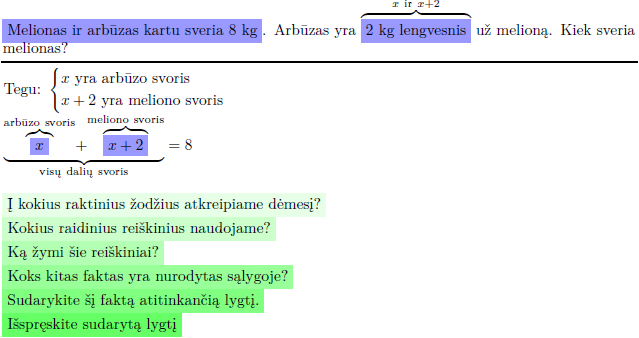
\includegraphics[width = \textwidth]{zodiniai.png}
\end{frame}

\begin{frame}[fragile]{Interaktyvaus aiškinimo pavyzdys}
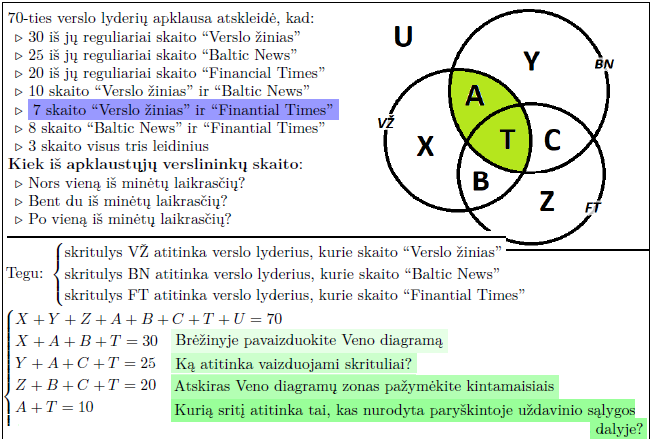
\includegraphics[width = \textwidth]{zodiniai2.png}
\end{frame}

\begin{frame}[fragile]{Sprendimų vaizdavimas su .pdf failais}
3. Prasmės pavaizdavimas reiškiniuose.
\begin{itemize}
\item Tikslas: ugdyti įprotį įsimenant matematinę medžiagą kreipti dėmesį ne tik į reikšmes, bet ir į prasmes.
\item Tipinis vadovėlinis klausimas: kokia reiškinio $x(x+1)$ reikšmė, kai $x=2?$
\item Mano klausimas: kokia šio reiškinio prasmė?
\end{itemize}
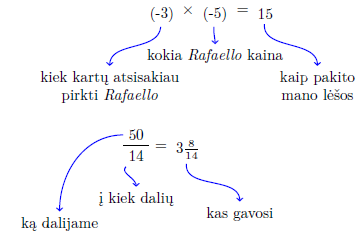
\includegraphics[width = 0.6\textwidth]{prasme.png}
\end{frame}

\begin{frame}[fragile]{Sprendimų vaizdavimas su .pdf failais}
4. Iššokančiosios užuominos.
\begin{itemize}
\item Tikslas: suteikti galimybę sprendimo aiškinimo gylį pasirinkti pačiam pagal poreikius.
\item Sprendimo žingsnių paaiškinimus galima klasifikuoti į atskirus tipus: įvedamų kintamųjų prasmės paaiškinimas, parodymas, kas įstatoma ir į kokią formulę, parodymas, kokia lygybe remiantis buvo atliktas pertvarkymas.
\end{itemize}
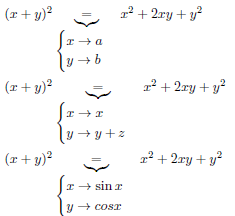
\includegraphics[width = 0.4\textwidth]{show.png}
\end{frame}

\begin{frame}[fragile]{Iššokančių užuominų pavyzdys}
Tekste galima talpinti kaip nors žymimus interaktyvius laukelius. 
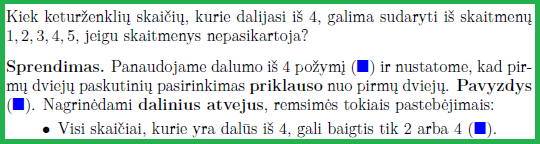
\includegraphics[width = 0.78\textwidth]{tooltips1.png}

Paspaudus ant pažymėtos teksto dalies iššoka užuomina:
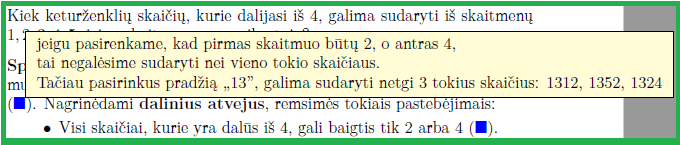
\includegraphics[width = \textwidth]{tooltips2.png}

Paspaudus dar sykį, užuominą išnyksta.
\end{frame}

\begin{frame}[fragile]{Sprendimų vaizdavimas su .pdf failais}
5. Animacijos.
\begin{itemize}
\item Tikslas: supaprastinti įvairius stebėjimus, pakeisti medžiagos formatą į lengviau įsisavinamą.
\item Galima rinktis du animavimo būdus: ar kadrus kursime su Python, ar su LaTeX.
\end{itemize}
\end{frame}

\begin{frame}[fragile]{Animacijų pavyzdžiai: Latex programavimas}
\newcounter{k}
\setcounter{k}{-15}

\begin{animateinline}[controls,autoplay,palindrome, poster = last, loop, begin={
  \begin{tikzpicture}[domain=-5:5,samples=100, scale=0.65]%
  %\useasboundingbox (0,-0.5) rectangle (0.5\textwidth, 0.75);
}, end={\end{tikzpicture}}]{10}%
  \whiledo{\thek<17}{%
    \draw[very thin,color=gray] (-4.9,-0.9) grid (4.9,0.9);%
    \draw[->] (-5.2,0) -- (5.2,0) node[right] {$x$};%
    \draw[->] (0,-1.5) -- (0,1.5) node[above] {$y$};%
    \pgfmathsetmacro\result{\thek/10};%
    \ifthenelse{\thek<0}{%
    \draw[thick, color=purple]   plot (\x,{sin(deg(\x+\thek/10)})    node[right, minimum height=0.7cm, minimum width=4cm] {$f(x) = \sin (x\pgfmathprintnumber{\result})$};}%
   {\draw[thick, color=purple]   plot (\x,{sin(deg(\x+\thek/10)})    node[right, minimum height=0.7cm, minimum width=4cm] {$f(x) = \sin (x+\pgfmathprintnumber{\result})$};}%
 % \end{tikzpicture}%
  \stepcounter{k}%
  \ifthenelse{\thek<17}{\newframe}{\end{animateinline}}}%
  \setcounter{k}{-15}
\begin{animateinline}[controls,autoplay,palindrome]{10}
  \whiledo{\thek<17}{%
  \begin{tikzpicture}[domain=-5:5,samples=100, scale=0.65]%
    \draw[very thin,color=gray] (-4.9,-2.9) grid (4.9,2.9);%
    \draw[->] (-5.2,0) -- (5.2,0) node[right] {$x$};%
    \draw[->] (0,-2.9) -- (0,2.9) node[above] {$y$};%
    \pgfmathsetmacro\result{\thek/10};%
    \ifthenelse{\thek<0}{%
    \draw[thick, color=purple]   plot (\x,{sin(deg(\x))+\thek/10})    node[right, minimum height=0.7cm, minimum width=4cm] {$f(x) = \sin (x)\pgfmathprintnumber{\result}$};}%
   {\draw[thick, color=purple]   plot (\x,{sin(deg(\x))+\thek/10})    node[right, minimum height=0.7cm, minimum width=4cm] {$f(x) = \sin (x)+\pgfmathprintnumber{\result}$};}%
  \end{tikzpicture}%
  \stepcounter{k}%
  \ifthenelse{\thek<17}{\newframe}{\end{animateinline}}}%
\end{frame}

\begin{frame}[fragile]{Animacijų pavyzdžiai: Latex programavimas}
\pgfmathsetmacro\myangle{0}
\def\angle{\myangle}
\begin{animateinline}[controls,autoplay,loop]{15}
\whiledo{\lengthtest{\angle pt<360pt}}{%
  \begin{tikzpicture}
    % fill circle and plot
    \fill[blue!50] (-1,0) arc (0:\angle:2) -- (-3,0) -- cycle; %goes to; startangle:initialangle:radius; goes from
    \fill[blue!50] plot[smooth,domain=0:\angle] (pi/180*\x,{2*sin(\x)}) |- (0,0);
    % draw connection
    \draw (-3,0) +(\angle:2) circle (4pt) -- (pi/180*\angle,{2*sin(\angle)}) circle (4pt);
    % draw axes an ticks
    \draw (-5.5,0) -- (7,0);
    \foreach \deg in {45,90,135,180,225,270,315,360}
      \draw (pi/180*\deg,2pt) -- (pi/180*\deg,-2pt) node[below] {$\deg^\circ$};
    \draw (0,-2.2) -- (0,2.2);
    \foreach \y in {-1,-0.5,0.5,1}
      \draw (2pt,2*\y) -- (-2pt,2*\y) node[left] {$\y$};
    %draw blue stick
    \draw[very thick, blue] (-3,0) +(\angle:2) circle (4pt) -- (-3,0);
    % draw plot and circle outline
    \draw plot[smooth,domain=0:360] (pi/180*\x,{2*sin(\x)});
    \draw (-3,0) circle (2);%
   \pgfmathsetmacro\myangle{\angle+5.0} %myangle cant be used globally
   \xdef\angle{\myangle} %we copy it to global variable
   \end{tikzpicture}
   \ifthenelse{\lengthtest{\angle pt<360pt}}{\newframe}{\end{animateinline}}   
}
\end{frame}

\begin{frame}[fragile]{Animacijų pavyzdžiai: Latex programavimas}
\pgfmathsetmacro\myangle{0}
\xdef\angle{\myangle}
\begin{animateinline}[controls,autoplay,loop]{15}
\whiledo{\lengthtest{\angle pt<360pt}}{%
  \begin{tikzpicture}
    % fill circle and plot
    \fill[blue!50] (-3,2) arc (90:\angle+90:2) -- (-3,0) -- cycle; %goes to; startangle:initialangle:radius; goes from
    \fill[blue!50] plot[smooth,domain=0:\angle] (pi/180*\x,{2*cos(\x)}) |- (0,0);
    % draw connection
    \draw (-3,0) +(\angle+90:2) circle (4pt) -- (pi/180*\angle,{2*cos(\angle)}) circle (4pt);
    % draw axes an ticks
    \draw (-5.5,0) -- (-5,0);
    \draw (-1,0) -- (7,0);
    \draw (-3,-2) -- (-3,2);
    \foreach \deg in {45,90,135,180,225,270,315,360}
      \draw (pi/180*\deg,2pt) -- (pi/180*\deg,-2pt) node[below] {$\deg^\circ$};
    \draw (0,-2.2) -- (0,2.2);
    \foreach \y in {-1,-0.5,0.5,1}
      \draw (2pt,2*\y) -- (-2pt,2*\y) node[left] {$\y$};
    %draw blue stick
    \draw[very thick, blue] (-3,0) +(\angle+90:2) circle (4pt) -- (-3,0);
    % draw plot and circle outline
    \draw plot[smooth,domain=0:360] (pi/180*\x,{2*cos(\x)});
    \draw (-3,0) circle (2);%
   \pgfmathsetmacro\myangle{\angle+5.0} %myangle cant be used globally
   \xdef\angle{\myangle} %we copy it to global variable
   \end{tikzpicture}
   \ifthenelse{\lengthtest{\angle pt<360pt}}{\newframe}{\end{animateinline}}   
}
\end{frame}

\begin{frame}[fragile]{Animacijų pavyzdžiai: Latex programavimas}
 \pgfmathsetmacro\myangle{0}
\xdef\angle{\myangle}
\begin{animateinline}[controls,autoplay,loop]{15}
\whiledo{\lengthtest{\angle pt<360pt}}{%
  \begin{tikzpicture}[scale=0.75]
    % fill circle and plot
    \path[use as bounding box] (-5.6,-4.7) rectangle (6.6,4.7);
    \ifthenelse{\lengthtest{\angle pt=90pt}}{}{
    \ifthenelse{\lengthtest{\angle pt=270pt}}{}{
    \fill[blue!50] plot[smooth,domain=0:1.5] (\x-3,{\x*tan(\angle)}) |- (0,0); %goes to; startangle:initialangle:radius; goes from
    \ifthenelse{\lengthtest{\angle pt<90pt}}{\fill[blue!50] plot[smooth,domain=0:\angle] (pi/180*\x,{1.5*tan(\x)}) |- (0,0);}{
    \fill[blue!50] plot[smooth,domain=0:85] (pi/180*\x,{1.5*tan(\x)}) |- (0,0);
     \ifthenelse{\lengthtest{\angle pt<270pt}}{\fill[blue!50] plot[smooth,domain=95:\angle] (pi/180*\x,{1.5*tan(\x)}) |- (9.5*pi/18,0);}{
     \fill[blue!50] plot[smooth,domain=100:265] (pi/180*\x,{1.5*tan(\x)}) |- (9.5*pi/18,0);
     \fill[blue!50] plot[smooth,domain=275:\angle] (pi/180*\x,{1.5*tan(\x)}) |- (27.5*pi/18,0);}}
    % draw connection
    \draw (-1.5,{1.5*tan(\angle)}) circle (3pt) -- (pi/180*\angle,{1.5*tan(\angle)}) circle (3pt);}}
    % draw axes an ticks
    \draw (-5.5,0) -- (7,0);
    \foreach \deg in {45,90,135,180,225,270,315,360}
      \draw (pi/180*\deg,2pt) -- (pi/180*\deg,-2pt) node[below] {$\deg^\circ$};
    \draw (0,-7.6) -- (0,7.6);
    \foreach \y in {-5,-4,-3,-2,-1,-0.5,0.5,1,2,3,4,5}
      \draw (2pt,1.5*\y) -- (-2pt,1.5*\y) node[left] {$\y$};
    %draw blue stick
    \draw[very thick, blue] (-3,0) +(\angle:1.5) -- (-3,0);
    % draw plot and circle outline
    \draw plot[smooth,domain=0:80] (pi/180*\x,{1.5*tan(\x)});
    \draw plot[smooth,domain=100:260] (pi/180*\x,{1.5*tan(\x)});
    \draw plot[smooth,domain=280:360] (pi/180*\x,{1.5*tan(\x)});
    \draw (-3,0) circle (1.5);%
   \pgfmathsetmacro\myangle{\angle+5.0} %myangle can't be used globally
   \xdef\angle{\myangle} %we copy it to global variable
   \end{tikzpicture}
   \ifthenelse{\lengthtest{\angle pt<360pt}}{\newframe}{
   \end{animateinline}
   }   
}
\end{frame}

\begin{frame}[fragile]{Animacijų pavyzdžiai: Python programavimas}
\newcounter{frameindex}
\setcounter{frameindex}{1}
Į kvadratą įbrėžiame apskritimą.

Padalijame šį kvadratą į $n \times n$ kvadratėlių.

Kvadratėlius, kurie yra vidinėje šio apskritimo dalyje, bet nėra kertami apskritimo, nuspalviname šviesiai mėlynai.

Kvadratėlius, kurie yra kertami apskritimo, nuspalviname tamsiai mėlynai.

Kurią dalį kvadrato sudaro mėlyni kvadratėliai?

\begin{animateinline}[controls,autoplay,loop]{2}
\whiledo{\theframeindex<100}{
  \begin{tikzpicture}
    \node[inner sep=0pt] (exc) at (0,0)
    {\includegraphics[width=\textwidth]{frames/exc\theframeindex.png}};
   \end{tikzpicture}
   \stepcounter{frameindex}
   \ifthenelse{\theframeindex<100}{\newframe}{\end{animateinline}}}

\setcounter{frameindex}{3}
\end{frame}

\begin{frame}[fragile]{Animacijų pavyzdžiai: Python programavimas}
Eksperimentas, kuris leidžia geriau įsivaizduoti, į ką panašėja figūra, gauta skritulį dalijant į vis daugiau lygių dalių:
\begin{animateinline}[controls,autoplay,loop]{2}
\whiledo{\theframeindex<100}{
  \begin{tikzpicture}
    \node[inner sep=0pt] (ctos) at (0,0)
    {\includegraphics[width=\textwidth]{frames/ctos\theframeindex.png}};
   \end{tikzpicture}
   \stepcounter{frameindex}
   \ifthenelse{\theframeindex<100}{\newframe}{\end{animateinline}}}
\end{frame}
 
 \begin{frame}[fragile]{Animacijų pavyzdžiai: animuoti pertvarkymai su LaTeX}
\begin{animateinline}[controls, poster = last, loop, begin={
  \begin{tikzpicture}
  \useasboundingbox (0,-0.5) rectangle (\textwidth, 0.75);
}, end={\end{tikzpicture}}]{1}
$\sinh x = x + \frac {x^3} {3!} + \frac {x^5} {5!} + \frac {x^7} {7!} +\cdots $
\newframe
$2a\sinh x = 2ax + \frac {2ax^3} {3!} + \frac {2ax^5} {5!} + \frac {2ax^7} {7!} +\cdots =$
\newframe
$2a\sinh \left(\frac{x}{a}\right) = 2a\left(\frac{x}{a}\right) + \frac {2a\left(\frac{x}{a}\right)^3} {3!} + \frac {2a\left(\frac{x}{a}\right)^5} {5!} + \frac {2a\left(\frac{x}{a}\right)^7} {7!} +\cdots$
\newframe
$2a\sinh \left(\frac{x}{a}\right) = 2x + \frac{x^3}{3a^2} + \frac{x^5}{60a^4} +\cdots$
\newframe
$2a\sinh \left(\frac{S/2}{a}\right) = 2(S/2) + \frac{(S/2)^3}{3a^2} + \frac{(S/2)^5}{60a^4} +\cdots$
\newframe
$2a\sinh \left(\frac{S/2}{a}\right) = S+ \frac{S^3}{24a^2} +\cdots$
\end{animateinline}

\begin{animateinline}[controls, poster = last, loop, begin={
  \begin{tikzpicture}
  \useasboundingbox (0,-0.5) rectangle (\textwidth, 0.75);
}, end={\end{tikzpicture}}]{1}
$\cosh x = 1 + \frac {x^2} {2!} + \frac {x^4} {4!} + \frac {x^6} {6!} + \cdots$
\newframe
$a\cosh x = a + \frac {ax^2} {2} + \frac {ax^4} {24} + \frac {ax^6} {720} + \cdots$
\newframe
$a\cosh \left(\frac{S/2}{a}\right)  = a + \frac {a\left(\frac{S/2}{a}\right) ^2} {2} + \frac {a\left(\frac{S/2}{a}\right) ^4} {24} + \frac {a\left(\frac{S/2}{a}\right) ^6} {720} + \cdots$
\newframe
$a\cosh \left(\frac{S/2}{a}\right)-a  = \frac{S^2}{8a} + \cdots$
\end{animateinline}
\end{frame}

\begin{frame}[fragile]{Sprendimų vaizdavimas su .pdf failais}
6. Kiti nesudėtingi triukai, išskiriantys Latex iš kitų priemonių:
\begin{itemize}
\item Nuorodų įkėlimas. Pvz. galime tam tikrus pertvarkymus pasitikrinti internete:

\href{https://www.wolframalpha.com/input/?i=(y+or+not(z)+implies+z+and+not(x+and+y))+or+(x+equivalent+z)}{\textit{Pasitikrinkime, ar teisingai darėme}}
\item Skripto talpinimas.
\begin{minted}{python}
for i in range(3): 
	skaiciai = np.sqrt(skaiciai)
plt.plot(np.linspace(0,10,100), skaiciai)
\end{minted}
\end{itemize}
\end{frame}

\begin{frame}[fragile]{Sprendimų vaizdavimas su .pdf failais}
\begin{itemize}
\item Lygčių lygiavimas. Leidžia aiškiau matyti pertvarkymus.

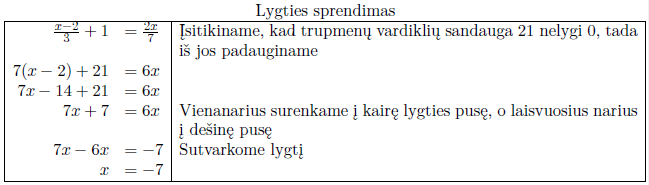
\includegraphics[width = \textwidth]{lygtys.png}
\end{itemize}
\end{frame}

\begin{frame}[fragile]{Sprendimų vaizdavimas su .pdf failais}
\begin{itemize}
\item Tekstas rėmeliuose. 
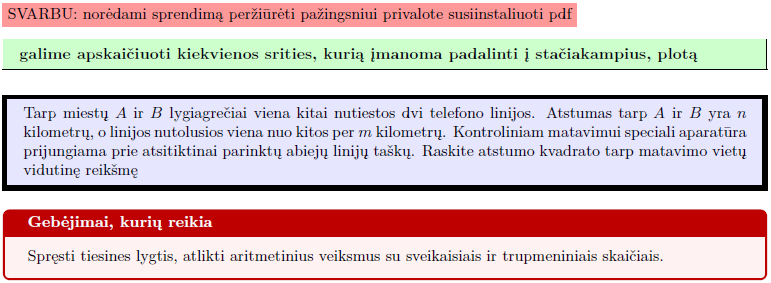
\includegraphics[width =0.9 \textwidth]{remai.png}
\item Interaktyvus turinys. Leidžia įeiti į pasirinktą temą
\end{itemize}
\end{frame}

\begin{frame}[fragile]{Vaizdavimo privalumai ir trūkumai}
\begin{itemize}
\item Darbo rezultatas padeda daug matematinės medžiagos vizualizuoti. Tai yra puiki pagalbinė priemonė norint aiškiai ir įsimenamai atsakyti į pagrindinius mokymosi klausimus: kaip pasikeis teiginio (reiškinio, lygybės, figūros...) forma taikant samprotavimo žingsnį, kaip pasikeis vieno kintamo objekto (reiškinio, teiginio, grafiko, figūros, lygybės) forma keičiant kitą objektą.
\end{itemize}
\end{frame}

\begin{frame}[fragile]{Vaizdavimo privalumai ir trūkumai}
\begin{itemize}
\item Rezultatą sunku pasiekti: daugybę techninių klausimų išsiaiškinti trunka per daug laiko. LaTeX yra redaktūros, o ne programavimo įrankis, todėl animacijų kūrimas yra labai sudėtingas. 

\item Dviejų skriptų pavyzdys: \href{https://pastebin.com/0qxQCsf7}{\texttt{Tangento animacijos su LaTeX}} ir \href{https://pastebin.com/YXVx8XT7}{\texttt{skritulio ploto animacijos su Python}}.

\item Abu skriptai reikalauja pradinių žinių, kaip naudotis specialiais paketais ir jų komandomis, skirtomis ,,patalpinti'' įvairius objektus į atskirus paketus. Šios žinios yra įgyjamos praleidžiant daug laiko skaitant tų paketų dokumentacijas.
\end{itemize}
\end{frame}

\begin{frame}[fragile]{Vaizdavimo privalumai ir trūkumai}
\begin{itemize}
\item Skirtumas tarp programavimo būdų: Python komandų arsenalas ne toks didelis ir lengviau perprantamas įprastam programuotojui, o dirbant su LaTeX reikia kur kas daugiau laiko praleisti aiškinantis klausimus, kurie įprastame programavime nekiltų. Laiko nuostoliai dideli.
\item Pavyzdys: kodėl ši komanda neveikia?
\begin{minted}{text}
\begin{mybox}{Gebėjimai, kurių reikia}
Spręsti tiesines lygtis, atlikti aritmetinius veiksmus su sveikaisiais ir trupmeniniais skaičiais.
\end{mybox}
\end{minted}
Atsakymas: 

\mintinline{text}{Gebėjimai, kurių reikia} reikėjo pakeisti į \mintinline{text}{Gebėjimai\text{,} kurių reikia}
\end{itemize}
\end{frame}

\begin{frame}[fragile]{Vaizdavimo privalumai ir trūkumai}
\begin{itemize}
\item LaTeX: pagrindiniai laiko nuostoliai dirbant kyla dėl neinformatyvių klaidų pranešimų.  Pvz. pranešimas:
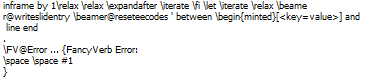
\includegraphics[width =0.9 \textwidth]{pranesimas.png}
\item Kuriant animacijas kadrų apdorojimas lėtas. Pvz. vien ši pateiktis yra apdorojama tik per 2 minutes dėl didelio animacijų kiekio.
\item Norint išgauti tam tikras galimybes reikia aiškintis daug pašalinių klausimų. Pvz. skriptų rodymas ir iššokančiosios užuominos neveiks leidžiant skriptą per kitus kompiuterius, neturinčius tų pačių nustatymų. Be to, animacijas ir užuominas galima matyti tik per Adobe Acrobat Reader.
\end{itemize}
\end{frame}

\begin{frame}[fragile]{Vaizdavimo privalumai ir trūkumai}
Išvados: LaTeX patogus naudoti tik paprastoms, su teksto redagavimu susijusioms užduotims. Jei norime kurti animacijas ir paveisklėlius, laiko prasme kadrus geriau kurti su programavimo kalba. 
\end{frame}

\begin{frame}[fragile]{Alternatyvos LaTeXui: .md formatas}
\begin{itemize}
\item .md failų formatas - tai formatas, pritaikytas įvairių programų dokumentacijoms. 
\item Jo redaktūra yra supaprastinta. 
\item \texttt{README.md} failas yra įprastinė kiekvieno programavimo projekto dalis.
\item Skaitymui ir redagavimui galima naudoti redaktorius, tokius kaip \texttt{Typora}{https://typora.io}.
\item Geras pavyzdys yra \href{https://npm.pkg.github.com/Nimmel/Python}{čia}.
\item Kompiliavimas neužtrunka, tačiau failą perkėlus į kitą kompiuterį, iliustracijų nesimatys, nes bus prarastos jų nuorodos.
\end{itemize}
\end{frame}

\begin{frame}[fragile]{Alternatyvos LaTeXui: .md sintaksė}
\begin{itemize}
\item .md failų formatas - tai formatas, pritaikytas įvairių programų dokumentacijoms. 
\item Jo redaktūra yra supaprastinta. 
\item \texttt{README.md} failas yra įprastinė kiekvieno programavimo projekto dalis.
\item Skaitymui ir redagavimui galima naudoti redaktorius, tokius kaip \texttt{https://typora.io}{Typora}.
\item Geras pavyzdys yra \href{https://npm.pkg.github.com/Nimmel/Python}{čia}.
\item Kompiliavimas neužtrunka, tačiau failą perkėlus į kitą kompiuterį, iliustracijų nesimatys, nes bus prarastos jų nuorodos.
\end{itemize}
\end{frame}

\begin{frame}[fragile]{Alternatyvos LaTeXui: .md formatas}
\begin{itemize}
\item Lentelės
\begin{minted}{md}
| First  | Second |
| :----: | :----: |
| plan A | plan B |
\end{minted}
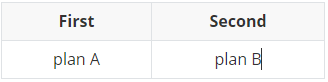
\includegraphics[width=0.6 \textwidth]{lenteles.png}
\end{itemize}
\end{frame}

\begin{frame}[fragile]{Alternatyvos LaTeXui: .md formatas}
\begin{itemize}
\item Paveikslėlių įkėlimas
\begin{minted}{md}
![](readme_image.png) 
\end{minted}

\includegraphics[width=0.3 \textwidth]{not_slight.png}
\item Antraščių dydis reguliuojamas grotelėmis prieš tekstą.
\item Pasvirimas, paryškinimas ir sąrašo sudarymas reguliuojami * simboliais.
\end{itemize}
\end{frame}

\begin{frame}[fragile]{Programavimas gyvai}
Mokiniams atrodo sudėtinga įvairias matematines užduotis atlikti kompiuteriu, pvz. :
\begin{itemize}
\item pažymėti koordinačių plokštumos taškus
\item nubraižyti stulpelinę diagramą
\item nustatyti skaičiaus daliklius
\item išrašyti visas įmanomas elementų poras iš 2 aibių
\end{itemize}
\end{frame}

\begin{frame}[fragile]{Programavimas gyvai}
Kas bendra tarp šių uždavinių?
\begin{itemize}
\item Kam daugiausiai gali būti lygus stačiakampio plotas, jei jo perimetras lygus 8?
\item Apytiksliai įvertinkite skaičių, kurį sudauginę su savimi 12 kartų gausite 2.
\item Su kuriuo N dešimtainis skaičiaus 1/N užrašas turės pabaigą?
\item Kaip pasikeis rezultatas, jei dalmenį sumažinsime 3 kartus?
\item Kiek yra dviženklių skaičių?
\item Kaip keisis rezultatas iš jo daug kartų traukiant šaknį?
\item Ar šaknų iš skaičių sandauga lygi šakniai iš skaičių sandaugos?
\end{itemize}
\end{frame}

\begin{frame}[fragile]{Programavimas gyvai}
Tipinė sprendimo struktūra:
\begin{itemize}
\item Kas tai yra? Ar galime rasti pavyzdžių?
\item Ar galime iš rastų pavyzdžių pastebėti dėsningumą?
\item Ar galime patikrinti, kiek pastebėtas dėsningumas atitinka tiesą?
\item Ar galime paaiškinti, kodėl dėsningumas galioja?
\end{itemize}
\end{frame}

\begin{frame}[fragile]{Programavimas gyvai}
Tipinė sprendimo struktūra (paryškinti klausimai gali būti lengviau atsakomi naudojant programavimą):
\begin{itemize}
\item Kas tai yra? Ar galime rasti pavyzdžių?
\item \textcolor{green}{Ar galime iš rastų pavyzdžių pastebėti dėsningumą?}
\item \textcolor{green}{Ar galime patikrinti, kiek pastebėtas dėsningumas atitinka tiesą?}
\item Ar galime paaiškinti, kodėl dėsningumas galioja?
\end{itemize}
\end{frame}

\begin{frame}[fragile]{Programavimas gyvai}
\begin{minted}{python}
skaiciai = np.linspace(0,2,100)
for i in range(3): skaiciai = np.sqrt(skaiciai)
plt.plot(np.linspace(0,10,100), skaiciai)
plt.show()
\end{minted}
\end{frame}

\begin{frame}[fragile]{Programavimas: už ir prieš}
\begin{itemize}
\item Programavimas padeda suvokti, jog svarbu ne tik kintamieji, bet ir jų kategorijos taip, kaip ir matematikoje.
\item Mokiniai nėra įpratę prie aukščiau minėtų samprotavimo žingsnių
\item Kai kurios loginės konstrukcijos per sudėtingos. Pvz. kuo skiriasi dviejų skaičių sumos kvadratas nuo jų kvadratų sumos?
\item Būtinas, nes dirbtinis intelektas \href{https://www.youtube.com/watch?v=wL7tSgUpy8w}{ima pranokti vaikus}
\end{itemize}
\end{frame}


\end{document}

